\chapter{Related Work}
This chapter will give an overview into the background and concepts of this thesis.
In the first section the Internet of Things an related subtopics like Smart Factories and Smart Cities are considered.
Cyber Physical Systems, which are important for the development of Smart Factories are also covered in this section.
Virtualization in general is the main topic of the second section.
First we dive into the area of Virtual Machines, followed by Container Virtualization.
Both are related to each other and sharing some basic ideas.
Container Orchestration as an own subsection show some possibilites of Container Virtualization.
The last subsection Network Function Virtualization concludes with an introduction into the virtualization of network node functions to create communication services.


\section{Internet of Things}


\subsection{Smart Factories}


\subsection{Cyber Physical Systems}


\subsection{Smart Cities}


\section{Virtualization}


\subsection{Virtual Machines}


\subsection{Container Virtualization}


\subsubsection{Docker}

"First, we must know what exactly Docker is and does. Docker is a container managment system that helps easily manage Linux Container (LXC) in an easier and unversal fashion. This lets you create images in virtual environment ons your laptop and run commands or operations against them. The actions you do to the containers that you run in these environments locally on your own machine will be the same commands or operations you run against them when they are running in your production environment. This helps in not having to do things differently when you go from a development environment like that on your local machine to  a production environemnt like that on your local machine to a production environemnt on your server. Now, let's take a look at the differences between Docker containers and the typical virtual machine environments.

In the followin illustration, we can see the typical Docker setup on the right-hand side versus the typical VM setup on the left-hand side:
\begin{figure}
    \centering
    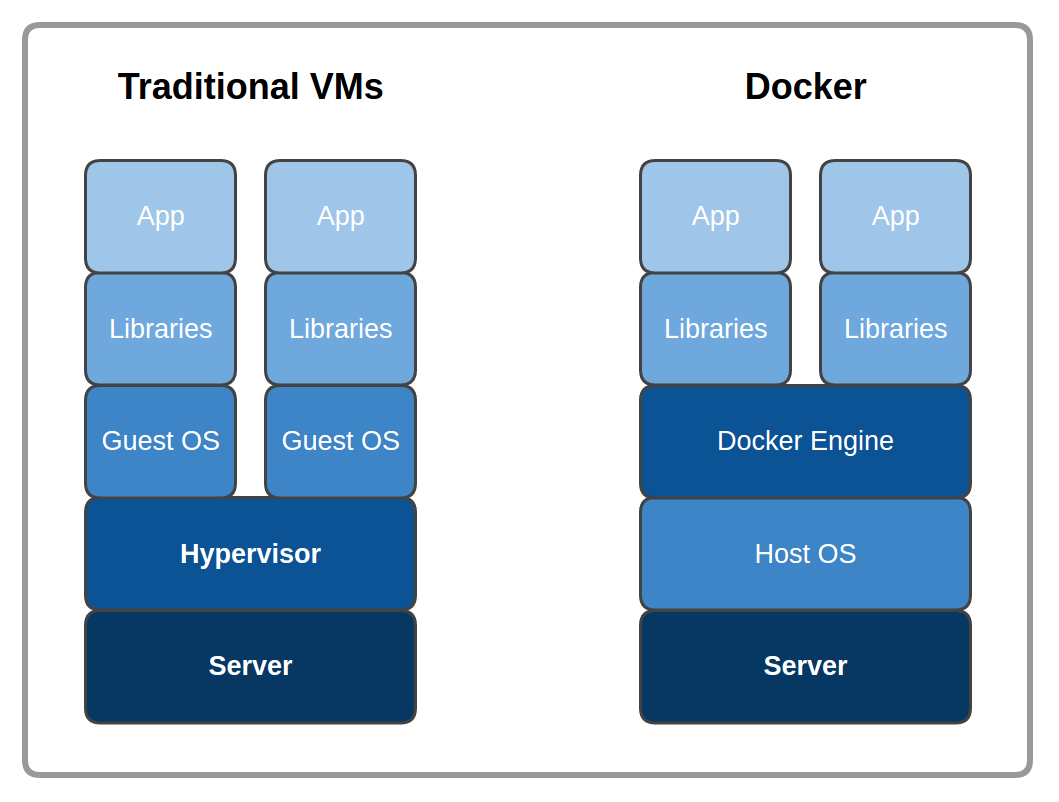
\includegraphics[width=0.6\textwidth]{resources/images//docker_vs_vm.png}
    \caption[Structure traditional VMs vs. Docker]{Structure traditional VMs vs. Docker. Adapted from: \cite{Gal2015}, p. 2}
    \label{fig:vms_vs_docker}
\end{figure}

This illustration gives us a lot of insight into the biggest key benefit of Docker, that is, there is no nedd for a complete operating system every titme we need to bring up a new container, which cuts down on the overall size of containers. Docker relies on using the host OS's Linux kernel (since almost all the versions of Linux use the standard kernel models) fot he OS it was build upon, such as Red Hat, CentOS, Ubuntu, and so on. For this reason, you can have almost any Linux OS as your host operationg system (Ubuntu in the previous illustartion) and be able to layer other OSes on top of the host. For example, in the earlier illustration, we could have Red Hat running for one app (the one on the left) and Debian running for the other app (the on on the right), but there would never be need to actually install Red Hat or Debian on the host. Thus, another benefit of Docker ist the size of aimages when they are born. They are not build with the largest piece: the kernel or the operating sytem. This makes them incredibley small, compact, and easy to ship."\cite{Gal2015}


\subsection{Container Orchestration}

\subsubsection{Kubernetes}

\subsubsection{Docker Swarm}


\subsection{Network Function Virtualization}


\section{Conclusion}
